\documentclass[a4paper,10pt]{article}
\usepackage[utf8x]{inputenc}

\usepackage{times}

\usepackage[pdftex]{graphicx}
\usepackage{epstopdf}

\usepackage[english]{babel}

\usepackage{anysize}
\marginsize{2cm}{2cm}{1.5cm}{2cm}

\usepackage{tabularx}
\usepackage{amsmath, amssymb, latexsym}
\usepackage[colorlinks=true, urlcolor=blue, citecolor=red]{hyperref}
\usepackage{datetime}


\newcommand{\titulo}[2]{ \begin{titlepage}\begin{center}\vspace*{\fill}\textsc{\Huge #1}\\[5cm]\textsc{\Large \underline{#2}}\\[5cm]\emph{Realizado por:}\\ \textsc{Jacinto Arias Martínez}\\ \textsc{Adrián Sánchez López}\vspace*{\fill}\vfill\monthname[\the\month],\, \the\year\end{center}\end{titlepage}}

\newcommand{\p}[1]{\paragraph{\indent\textnormal{#1}}}



\begin{document}

 \titulo{ARTIFICIAL INTELLIGENCE IN VIDEOGAMES}{Videogame Analysis: Starcraft}

    \begin{abstract}
    
    \end{abstract}

  \newpage

  \vspace*{3cm}
  \tableofcontents
  \vspace*{\fill}

  \newpage


\section{Origins and repercussion}

    Starcraft is a popular RTS \footnote{RTS: Real Time Strategy} game developed by Blizzard Entertainment, released on 1998. As the previous Blizzard's popular RTS game \textit{Warcraft II}, Starcraft quickly became the \textit{de facto} standard for this kind of games; it is estimated that more than 11 millions of copies have been sold.

    \p{Starcraft works in PC platform both Windows and Mac OS, also a Nintendo64 version was published a few years later but it didn't became so popular by the lack of multiplayer system. A good welcomed expansion was published in the same year a few months later, adding a new campaign and new units. Also in 2010, the expected sequel \textit{Starcraft II: Wings of liberty}, came selling more than 1.5 million copies in the first 48 hours.}

    \p{Starcraft multiplayer has been one the most played games in the internet through the pioneer Blizzard's multiplayer platform \textit{Battle.net}. Starcraft can be considered one of the few games that people had been still playing more than 10 years after the release, maybe it has been only replaced by its sequel. The game's popularity has led to professional players and leagues with sponsorship and televised matches, specially in South Korea, where the game is really popular.}
  
  \begin{figure}[hbt]
  \begin{center}
  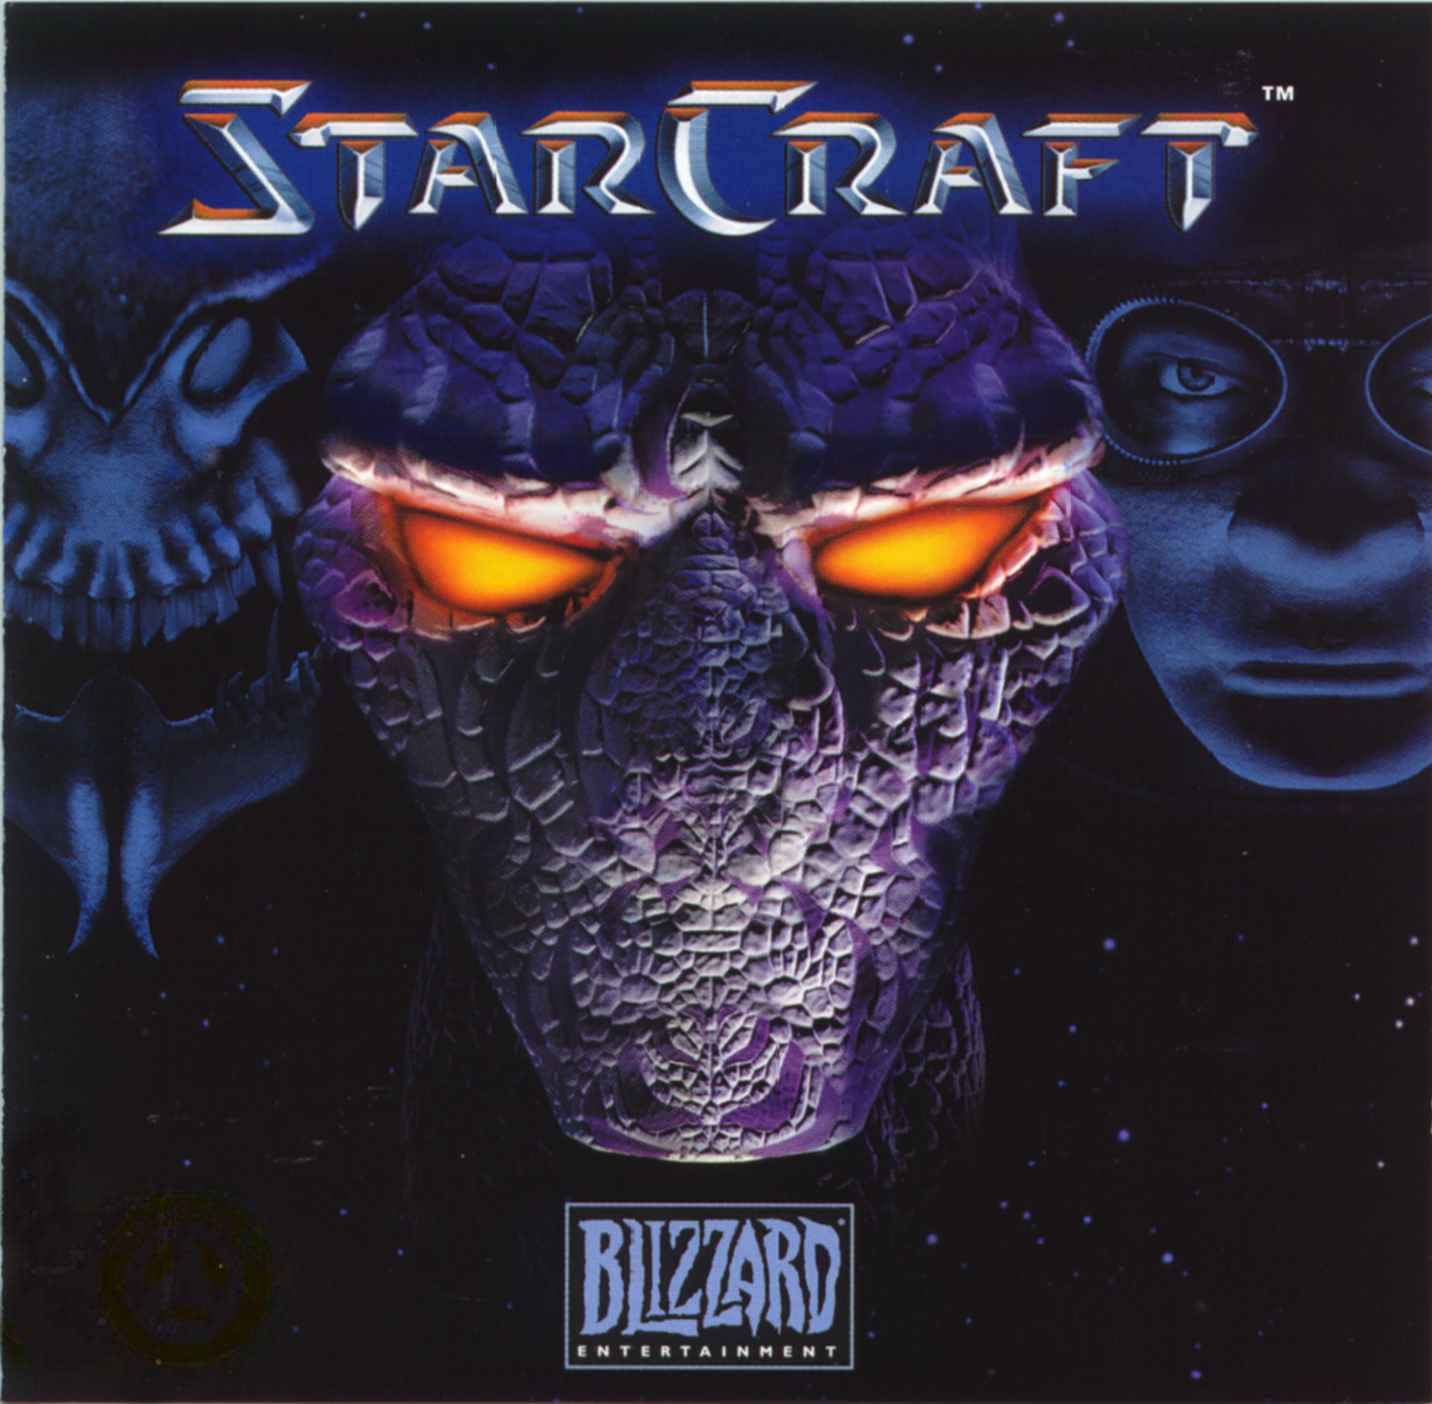
\includegraphics[scale=.5]{figs/logo.jpeg}
  \end{center}
  \caption{Starcraft original front.}
  \label{fig:rb1}
  \end{figure}

\newpage
\section{Features and gameplay}

  \p{In this section we will tell something about the game context and some of the game mechanic before starting a deeper analysis of the game, which should be pretty complex.}

  \subsection{The world of Starcraft}

    \p{Starcraft is based on a science-fiction world, where three races fight to take control of a solar system far away from the Earth. The three races are:}

    \begin{itemize}
     \item \textbf{Terran:} A technological advanced human society that long time ago moved from earth and get lost in space founding a new independent colony.
     \item \textbf{Protoss:} An elder alien race with advanced society and technology that has became in decadency.
     \item \textbf{Zerg Swarm:} An parasitic insectoid race of aggressive lifeforms that consume planets in order to assimilate the genetic of the native ones.
    \end{itemize}

    \p{Each race has a different tech tree, including many buildings and units for playing the game. Also, each race has their own capabilities which make a characteristic gameplay. So all your strategy will be conditioned to the race you and your opponents choose in each game.}

  
  \subsection{Game basics}

    \p{In order to defeat your opponents you will have to gather resources, build bases and armies and use them against your enemies.}

    \p{In your screen you will see a portion of the map, you will be able to move along by pushing the screen borders with your mouse. To control your units and buildings you can select them by pointing with your mouse, all you will be able to give them orders (either alone or in groups) by clicking in the right option in the menu or just with a keyboard or mouse shortcut.}

    \p{Your units will be able to walk to a different point of the map, to attack other units or patrol some areas. When a unit hasn't received any orders it will stay in its place attacking and chasing any enemy unit that enter its vision range.}

    \p{In Starcraft there are two different kind of games:}

    \begin{itemize}
     \item \textbf{Campaign mode:} Starcraft comes with a set of special maps in which the plot of the game is told to you as you go through them. Cinematic sequences and dialogues occur during this maps and the main goals of the maps are updated as the story goes along. This game mode is for one human player and all your opponents will be AI controlled players, each map initial configuration is set according to the plot circumstances.

    \item \textbf{Multiplayer mode:} This game mode is the most interesting for this work. In this game mode, players both human and computer controlled face each other, team working is supported and the goal is to defeat your opponents by destroying all their buildings. I this game mode, all players start in random predefined places of the map, next to a resources emplacement with the main building a 5 workers.
    \end{itemize}


\newpage
\section{Artificial intelligence principles I: Computational Theory}

  \subsection{Game elements}

    \p{In a standard Starcraft game, you will be placed in a map with different terrain configurations, including different heights, water, vast space, lava, jungle and much more. Also you will find necessary resources to gather. Other players will be placed and you will play with or against them in order to achieve the particular goal of the map. For this, you will have access to a particular set of units and building according to your race.}

    \p{Next we will introduce the different elements of the game in order to \textbf{establish a base of knowledge}:}

    \subsubsection{Map, terrain and visibility}

      \p{As we say, each game is played on a specific map. The terrain types condition how the units can move around the map, i.e a terran marine would walk on the normal ground but it's not allowed to move on the water or lava, however a flying unit will be able to move freely in every type of terrain.}

      \p{Normally, the map is covered in a black colour which represents that you've never visited this area with any unit. Also, there will be areas where the terrain is in a grey colour called \textit{war fog}, so you could not be able to see any of the enemy units in the area, this represents that none of your units can \textit{see} this area. Each unit has a different \textbf{vision range} which would determine the areas you will see; also, a non flying unit would not be able to see in any terrain higher than the one it is.}


    \subsubsection{Units}

      \p{Each race has its set of different units. Every unit in the game has an amount of health points, energy, amour and the majority of them has an attack with its own range and damage. You can find many different type of unit in the game, much of them have special abilities and special purposes, it's needed to use them properly to be a good player.}

      \p{Each unit is stronger to beat other kinds of units, and is weaker to other kind with no exception, so in order to defeat your enemy you will need to attack him with an optimal army depending of what he has.}

      \p{Also each race has a worker unit, which is the only unit with can build buildings and gather resources. They are cheap and weak and are the basis of the game economy.}

      \p{There is two type of units: ground units and air units. The first can only move on the normal terrain and just change to a higher level when using a ramp. The flying ones could move through every kind of terrain. The attack of each unit is defined for ground, air or ground-air targets so it means that some units could not be able to attack specific ones.}


    \subsubsection{Buildings}

      \p{A building is like a unit but unlike them are attached to ground and are unmovable (that's quite a lie because some of terran buildings can take of the ground and fly) and have a great amount of health points. The buildings purposes include: receiving the gathered resources, train units or do researching. Some structures are defensive so they can attack enemy units.}


    \subsubsection{Resources}

     \p{Units and buildings have a different cost of resources that you will need to you must have and pay in order to afford it. Resource is gathered from the map and instantly added to your actual amount. When you build or train units the cost will be subtracted from your amount. If you can't afford it the unit would not be trained and the game will tell you that you'll need more resource.}

     \p{The most common resource is the \textit{mineral}, that can be found in different places of the map in form of finite deposits, your workers will gather this until each deposit is finished (they will disappear). Another resource is the \textit{vespene gas}, it quantity is lower than the mineral and it's more complex to gather it, however the cost of the units in gas is usually lower.}

     \p{There is another special type of resource called \textit{population} resource. This resource is not gathered and it's not spent, in this case you will have to maintain a maximum level of this resource in order to build a larger army; each race obtains population resource from a different kind of building or unit.}



    \subsubsection{Researching and tech tree}

      \p{As said above, each race has an unique set of units and buildings. In order to obtain them the player should meet some prerequisites, commonly it has to build an specific building.}

      \p{Some building can do researches and upgrades in order to improve the units or give them a special ability. Each upgrade costs an amount of resources and takes a lot of time to be completed, but it can make a difference in the game.}

  \subsection{Game strategies}

    \p{Having identified the elements involved in a Stracraft game, it's time to talk about the different way to use them to play this game properly:}

    \begin{itemize}
     \item A solid economy is needed. You will have to explore to find new resources, expand your base and build enough workers to gather resource. A solid economy will allow to have a stronger army.
     \item Exploration is fundamental; when playing this kind of RTS game you should try to know what your opponent is doing at every moment. For this, you will need to continuously explore the map with the fastest units and spy the enemy bases to know which kind of units they have in order to make a proper army to beat them.
     \item Build your bases to properly defend them, use buildings and terrain to take advantage. You can place units behind buildings to defend them and delaying the enemy or place your defences on higher levels to stop the enemy. Also you should take care of the enemy flying units that could infiltrate your bases at any point.
     \item Harass your enemy and make all the economic damage you can. Killing the enemy units is a good point to start but if you don't kill its workers or important buildings he will recover faster and will counter-attack you. Look for defence breaks in order to do as much damage as you can minimizing yours.
    \end{itemize}



  \subsection{Artificial intelligence applications}

    \p{There are two elements in Starcraft which design can be focused in artificial intelligence:}

    \subsubsection{Artificial intelligence in the game's core}

      \p{As Starcraft don't use any advanced physics or 3d perspective to solve, the game core solve this kind of problem with design solutions rather than with complex algorithms.}

      \p{For the perspective, the view is configured in a 2D isometric perspective which do trick of making different terrain heights, shadows and other effects without 3D rendering. Also the units attack are so simple, since no trajectories are calculated for the ranged shoots, so the impacts are calculated this way: ``If a unit is in range of another, and this one shoots it, the unit get damaged''.}

      \p{On the other hand, the independent behaviour of each unit is a complex problem that must be solved using advanced techniques. For example:}

      \begin{itemize}
       \item When a player order a unit to move somewhere, it has to trace a path and follow it across the map avoiding terrain obstacles, buildings and other units. Also this behaviour gets complicated when more than one unit is doing this.
       \item Also, the units stand in an aggressive mode and have to decide which enemies to shoot when they are in range. Actually in the game, a unit will attack the most nearly enemy unit.
      \end{itemize}




    \subsubsection{Artificial intelligence as an opponent}

      \p{Whether in campaign or multiplayer mode, AI opponents could be added in order to control one of the players. This AI should be able to perform all the actions needed to play in the same way a human would do. This include using accordingly all the units of the race chosen, build its base, gather resources, exploring and in summary all the strategies that we told above.}

      \p{This could be two point of view of an AI controlling the game:}

      \begin{itemize}
       \item \textbf{Micro management:} Although the units can act by themselves, the player must order them more precisely if he want to take advantage of their opponents either in combat or moving a big army. We are speaking about micro management in the cases of ordering your units to directly attack other specific unit, when scouting the enemy bases or something that requires more precise control.

      \item \textbf{Macro management:} We speak about macro management when we tell about the player ability to produce units, and keep all of your production buildings busy. Generally, the player with the better macro will have the larger army. The other element of macro is your ability to expand at the appropriate times to keep your production of units flowing. A good macro player is able to keep increasing his or her production capability while having the resources to support it.

      Macro management is about taking decisions during the game and implementing your strategy by your actions. 
      \end{itemize}


    \subsection{Knowledge extraction}

      \p{Now that we have identified the elements involved in the game, so we know the domain, and we have also identified the needs for Artificial Intelligence applications, we should analyze different sources in order to extract and express knowledge and information in natural language; thereby we could apply in the future for choosing and developing our representation scheme.}

      \p{There are many sources from where we can extract the required knowledge such as: specific game guides, user experience, databases with stored games even classic strategy books which could give us a theory-based approach to solve the problem (like Sun Tzu's Art of War).}

      \p{For this work, we will focus on the second approach, covering just the case of the AI as an opponent. In the next paragraphs we will introduce specific techniques which should be used in order to play starcraft to a high competitive level with an abstraction level enough to be imported into any convenient representation system to permit an AI to use them.}

      \subsubsection{Economic issues}
	\begin{itemize}
	\item \textbf{You have to keep a minimum number of workers for each resource deposit:} In order to optimally gather resources, you will need 3 workers per deposit. So you will need to keep building them until you reach the needed number.

        \item \textbf{You have to balance your resources and production buildings:} Keeping large amounts of resources is a bad strategy. You must be able to spend all the resources you gather either training troops or expanding your base, so you will have to maintain enough production buildings in order to keep them busy and invest your resources. Unbalancing this, and having stopped production buildings  is also bad, so keep the everything balanced in every moment.

	\item \textbf{Expand your base once early and keep expanding during the game:} You should make an expansion at your first chance. You shouldn't be afraid of expanding yourself along the map because you will achieve profit immediately and defending expansions can be done dynamically. If one player has earlier expansions than their opponents, he could get a lot of advantage in a short time even if some of their expansions get destroyed.

	\item \textbf{Research every time you can afford it:} Researching costs a lot of time and you will get a lot of profit for all the units that you have been already trained. Researching could give a lot of advantage to a player if he overcomes his opponents in this field.

	\end{itemize}


  \subsubsection{Exploration and map positioning}


    \p{When you start a match, the map will be covered with a black colour which represents that you've never been at this area with any unit. Also, the areas where you have been but you don't have any unit at the moment will be covered with a transparent grey colour which represent that you won't see any enemy units at this place, this is the so called fog of war.}

    \p{As said before, in this game you should explore the map continuously in order to track your enemy activity.}

    \begin{itemize}
     \item \textbf{Keep exploring the map from the beginning to the end:} At the beginning of the map, you should send workers to explore the map, in order to localize your enemy and the resources deposit to later expand your base. Also, your should try to cover all the possible area, in order to know the map dispose.
     \item \textbf{Spy your enemies:} Also you should send units to your enemy bases and places where him should probably expanded. With this units, you should be able to discover his army, defences in order to use this information as a weak point. Attacking him in places poorly defenced, where his army is far away o to build an optimized army to beat his. Some kind of units are perfect for spying purposes, such as invisible ones, flying scouting units and so on.
     \item \textbf{Use the terrain properties:} We've said that you can find different types of terrains in the game, and you should take benefit of them. For example,  in most of map you will find ``islands'', which are places that cannot be reached by ground units; if you develop transports to move your workers and troops to this islands you can expand there in order to make a difficult expansion to find or to attack. Also your should take profit of the high terrain, because ground units can't climb to it unless there is a ramp, and neither they can see what is up there, so you can place long range units to kill the enemy units without been counter-attacked and also you can block the ramps to make your enemy get stuck in a bottle neck.
    \end{itemize}

  \subsubsection{Follow an optimal construction plan}
   
    \p{You shouldn't definitely not train or build every type of unit. In case of that, you should make a construction plan from the beginning of the game and you should evolve this if the situation require it. Following this construction plan will optimize either your resources and your strategy, saving you a lot of time and rushing your enemy. The construction plan should be used in order to implement your strategy.}

  \subsubsection{Use units properly}

     \p{We've said that every unit in the game is stronger in order to kill some kind of unit, and in the opposite side is weaker to another unit. That's true, but in the practice it becomes more complex, it is because you are able to combine different types of units in your army, and they will both have a different potential. Also, some units have special abilities which can change the course of a battle.}

     \p{Knowing all units strong points and weaknesses, so when you spy your enemy you will be able to decide which units are the most correct to train. Advanced human players know all of this by themselves and can determine if one type of unit is optimal in order to face others; an AI should be able to recognize this, and also it will be useful to store all the units different stats in order to calculate possible relations between units types by itself.}

  \subsubsection{Micro management: attacking and moving}

    \p{By default, a unit will attack the nearest enemy unit and will in the most straight that it could found. When you are facing a group of enemies, or you are moving large groups of them this is not by far the best approach to do that. Professional players prefer to direct command their troops to move or attack to specific places or units and they optimize so much their gameplay. It's true that a good micro management should win a battle which started in the same conditions.}

    \p{In order to optimize the movement, the professional players achieve a large numbers of mouse clicks per second in order to smooth the paths that the units follow and avoid the collision between them. This way, the different groups of units should be faster and have a better manoeuvrability.}

    \p{To take advantage of micro controlling on battles, the professional player order their units to focus fire on the strongest units to take them down faster and minimizing the fire that they could inflict to their troops.}

\subsection{Analysis of the different techniques: Identifying problems}

  \subsubsection{Heuristic search}

    \p{Heuristic search search could be applied in two ways:}

    \begin{itemize}
     \item It's a good approach to found paths for the micro-controlling of the different units. By executing really short searches in the near space the units should be able to navigate the map without colliding each other and smoothing the curves when avoiding obstacles.
     \item On the other hand, we can find heuristic search useful in order to make plans for the macro-controlling of the AI opponent. For example, we can search thought the space of different construction plans in order to adjust the current to the game status, where we can know about the enemy army or the different topology of the terrain.
    \end{itemize}

  \p{Heuristic search is not a good approach for direct controlling or more complex decisions because the combinatorial of the states will explode and be computationally unaffordable.}




\newpage
\section{Artificial intelligence principles II: Representation and algorithms}

    \p{In this section we will take further the above analysis in order to propose and design AI based solutions to comply the needs of the game.}

    \subsection{AIIDE 2010 StarCraft AI Competition}

      \p{First, we like to introduce this section talking about this event where Starcraft was proposed as a test platform to test the latest AI techniques. In this contest, sponsored by Stanford's University and Blizzard Entertainment, more than 60 groups of students of the most important universities competed developing different AI for Stracraft.}

      \p{The most interesting challenge were the matches between AI's, also, the more advanced played against one of the best human Starcraft players. None of them could be able to win, although they put the champion in a trouble.}

      \p{The competition included micro management battles, reduced technology battles and full Starcraft games battles. Some of the technologies used were:}

      \begin{itemize}
       \item Finite state machines
       \item Scripting
       \item Dynamic scripting
       \item Probabilistic inference
       \item Influence maps
       \item Neural networks
       \item Swarm intelligence
       \item Potential fields
       \item Genetic programming
      \end{itemize}

      \p{An API for programming AI in Starcraft is public available.}

\subsection{Heuristic search}

  \p{As said before, we can think about this technique in two ways.}

  \subsubsection{Input and output spaces}

    \p{If we are talking about micro management, and we want to make plans to move our units, our input spaces will be the coordinates of the units, and the topology of the map. The output will show the optimal path for the next movement. This search will be executed many times, as the movement of the units appears to be a continuous space.}

    \p{If we are talking about macro management, the input space will be our current army, economical data and other factors achieved during the exploration (terrain features and enemies information). The output space will be a construction plan for the next stage of the game.}


  \subsubsection{States}

  \subsubsection{Initial state – Final state}
\subsubsection{Operators}
\subsubsection{Function of heuristic evaluation}
\subsubsection{Search Techniques}
\end{document}          
